\documentclass[systemskiss/skiss.tex]{subfiles}
\begin{document}
\section{Inledning}
Systemet som ska konstrueras är en autonom taxibil. Den ska kunna ladda in en godtycklig bana som uppfyller kraven och göra köruppdrag på denna. Konstruktionen ska delas upp i moduler för att gruppmedlemmarna enkelt ska kunna arbeta parallellt med olika delar, samt att delar ska vara lätta att byta ut om produkten går sönder eller behöver uppgraderas.

\begin{figure}[h]
    \centering
    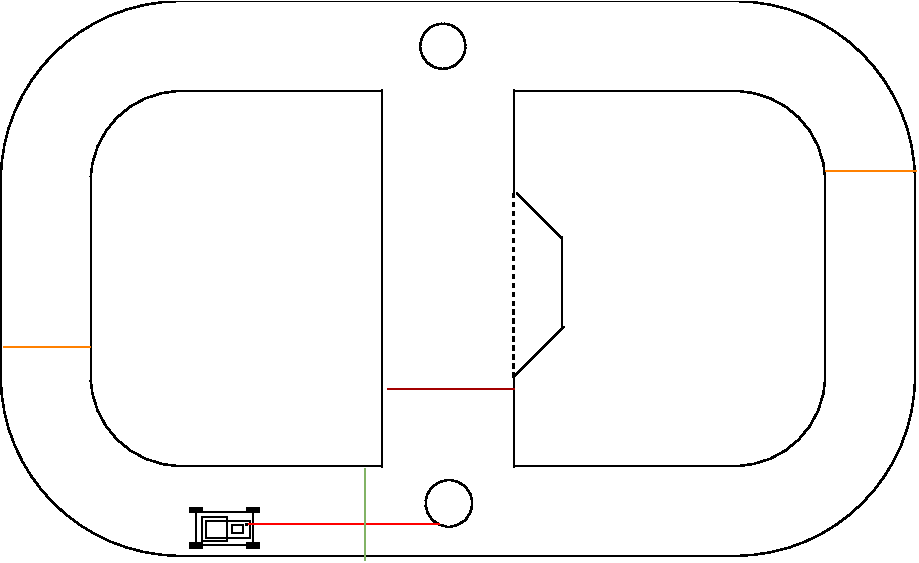
\includegraphics[width=0.6\linewidth]{systemskiss/figures/systemomgivning.pdf}
    \caption{Bild av systemet i dess omgivning}
    \label{fig:omgivning}
\end{figure}
\noindent
Figur \ref{fig:omgivning} visar när bilen är placerad i en bana så som det
skulle kunna se ut på tävlingen. Banan på bilden innehåller alla de komponenter
som banan kan innehålla. För mer exakt förklaring av banan se banspecifikationen.

\end{document}

